\documentclass[12pt,twoside,singlespace]{article}
\pagestyle{plain}

\usepackage{array, paralist, enumerate, amsmath, amsthm, amsfonts, amssymb, color, mathrsfs,comment}
%\usepackage{times}
\usepackage{geometry}
\usepackage{framed}
\usepackage{hyperref}
\usepackage{graphicx}
\usepackage{epstopdf}

\usepackage{tikz}
\usepackage{tkz-graph}
\usetikzlibrary{arrows,%
                shapes,positioning}

\definecolor{DarkBlue}{rgb}{0,0,0.8} 
\definecolor{DarkGreen}{rgb}{0,0.5,0.0} 
\definecolor{DarkRed}{rgb}{0.9,0.0,0.0} 

\usepackage[T1]{fontenc}
\usepackage[latin1]{inputenc}
%\usepackage[inline]{showlabels}

\numberwithin{equation}{section}
\newtheorem{thm}[equation]{Theorem}
\newtheorem{lem}[equation]{Lemma}
\newtheorem{cor}[equation]{Corollary}
\newtheorem{prop}[equation]{Proposition}

\theoremstyle{definition}
\newtheorem{definition}[equation]{Definition}
\newtheorem{ex}[equation]{Example}	
\newtheorem{remark}[equation]{Remark}
\newtheorem{prob}{Problem}

\newcommand{\BB}{\mathbf{B}}
\newcommand{\ZZ}{\mathbf{Z}}
\newcommand{\NN}{\mathbf{N}}
\newcommand{\RR}{\mathbf{R}}
\newcommand{\QQ}{\mathbf{Q}}
\newcommand{\CC}{\mathbf{C}}
\newcommand{\FF}{\mathbf{F}}
\newcommand{\N}{N}
\newcommand{\po}[2]{\mathfrak{po}^{#1|#2}}
\newcommand{\on}{\operatorname}
\newcommand{\ra}{\rightarrow}
\newcommand{\ul}{\underline}
\newcommand{\ol}{\overline}
\newcommand{\nin}{\noindent}

\newcommand{\simple}{\text{simple}}
\newcommand{\Img}{\on{Im}}
\newcommand{\con}{\on{Con}}
\newcommand{\dash}{\on{Dash}}

\geometry{verbose,letterpaper,tmargin=1in}

\newcommand{\Q}{\overline{q}}
\newcommand{\w}{\on{weight}}

\newcommand{\val}{\on{Val}}
\newcommand{\smon}{\mathbf{SMon}}
\newcommand{\clif}{\on{clif}}
\newcommand{\cl}{\mathbf{Cl}}
%\newcommand{\mov}[2]{\on{mov}_{#2}(#1)}
\newcommand{\inc}{\on{inc}}
\newcommand{\cut}[4]{#1 = #2 \amalg_{#4} #3}
\newcommand{\cutr}[3]{#1 \amalg_{#3} #2}
%\newcommand{\piece}[3]{#1(#2|#3)}
\newcommand{\piece}[3]{#1_{#3}}
\newcommand{\wt}{\on{wt}}

\newcommand{\com}[1]{\textcolor{red}{$[\star \star \star$ #1 $\star \star \star]$}}

%%%%%%%%%%%%%%%%%%%%%%%%%%%%%% LyX specific LaTeX commands.
%% Bold symbol macro for standard LaTeX users
\providecommand{\boldsymbol}[1]{\mbox{\boldmath $#1$}}

%%%%%%%%%%%%%%%%%%%%%%%%%%%%%% User specified LaTeX commands.
\renewcommand{\vec}[1]{\mathbf{#1}}

%\renewcommand{\labelenumi}{(\alph{enumi})}
%\renewcommand{\labelenumii}{(\roman{enumii})}

%\usepackage{babel}

\title{Study of lifting of 1D adinkras to 2D}
\author{Kevin Iga and Yan X Zhang}

\begin{document}

\pagestyle{plain}

\maketitle

\section{Preliminaries}

\subsection{$1$-d Adinkras}
Adinkras in [references] will be referred to as $1$-d Adinkras in this paper, since they relate to supersymmetry in $1$ dimension.  We will review a definition of $1$-d Adinkras now.  Note that while it is conventional to specify a natural number $N$ to denote the number of supersymmetries, we break with convention and instead specify $C$, a set of $N$ different colors.

\begin{definition}
Let $N$ be a non-negative integer.  A $1$-d Adinkra with $N$ colors is $(V,E,\chi,\Delta,g)$ where
\begin{itemize}
\item $V$ is a finite set of vertices
\item $E\subset V\times V$ is a set of edges
\item $\chi:E\to \{1,\ldots,N\}$ is a map called the coloring
\item $\Delta:E\to \{1,-1\}$ is a map called the dashing
\item $g:V\to\ZZ$ is a map called the grading
\end{itemize}

These are required to satisfy the following:
\begin{itemize}
\item If $(v,w)\in E$, then $(w,v)\in E$.  Furthermore, $\chi(v,w)=\chi(w,v)$ and $\Delta(v,w)=\Delta(w,v)$.
\item For every $v\in V$ and $c\in \{1,\ldots,N\}$, there exist exactly one $w\in V$ so that $(v,w)\in E$ and $\chi(v,w)=c$.
\item If $c_1$, $c_2\in C$ with $c_1\not=c_2$, and $v\in V$, then there exist $w$, $x$, and $y\in V$ so that $(v,w)$, $(w,x)$, $(x,y)$, and $(y,v)\in E$, and $\chi(v,w)=\chi(x,y)=c_1$ and $\chi(w,x)=\chi(y,v)=c_2$ and $\Delta(v,w)\Delta(w,x)\Delta(x,y)\Delta(y,v)=-1$.
\item If $(v,w)\in E$, then $|g(v)-g(w)|=1$.
\end{itemize}
\end{definition}
Note that in [Reference], there is also a bipartition of the vertices.  This is rendered obsolete by the grading, since $g(v)$ is even if and only if $v$ is a boson.

Recall that a $1$-d adinkra has a code $L(A)$, which is necessarily doubly-even. The code has parameters $(n,k)$, where $n$ is the number of coordinates and $k$ is the dimensions of the code. In this situation, the vertices of $A$ are labeled by cosets $\{0,1\}^n + L(A)$, so $|V(A)| = 2^{n-k}$.


Let $A$ be a $1$-d Adinkra with $N$ colors, with vertex set $V$.  For all $1\le i\le N$, define
\[q_i:V\to V\]
so that for all $v\in V$, $q_i(v)$ is the unique vertex joined to $v$ by an edge of color $i$.

Note that for all $v\in V$, $q_i(q_i(v))=v$ and $q_i(q_j(v))=q_j(q_i(v))$.  As a result, we can then define an action of $\ZZ_2^N$ on $V$ in the following way:
\[(x_1,\ldots,x_N)v=q_1^{x_1}\circ\cdots\circ q_N^{x_N}(v)\]

Pick a vertex $v\in A$.  Define $C(A,v)$ to be the stabilizer of $v$ under this action of $\ZZ_2^N$.  Since it is a subgroup of $\ZZ_2^N$, $C(A,v)$ is a binary block code of length $N$.

\begin{prop}
The Adinkra $A$ is connected if and only if the $\ZZ_2^N$ action is transitive on $V$.
\end{prop}
\begin{proof}
Let $v$, $w$ be vertices in $V$.  If $A$ is connected, then there is a path in $A$ connecting $v$ to $w$.  The edges in this path have colors $c_1,\ldots,c_k$.  Then $q_{c_1}\cdots q_{c_k}(v)=w$.  By the commutativity of $\ZZ_2^N$, we can rearrange $q_{c_1}\cdots q_{c_k}$ to be in increasing order of $c_i$.  This is then of the form $q_1^{x_1}\circ \cdots \circ q_N^{x_N}$ for some $(x_1,\ldots,x_N)\in \{0,1\}^N$.
\end{proof}

\begin{prop}
If $A$ is connected, then the code $C(A,v)$ does not depend on $v$.
\end{prop}
\begin{proof}
Let $w\in V$.  By the previous proposition, there exists $h\in \ZZ_2^N$ so that $hv=w$.

The result follows from the sequence of equivalences:
\[gw=w\leftrightarrow ghv=hv \leftrightarrow hgv=hv \leftrightarrow gv=v\]
\end{proof}
Thus, from now on we will refer to the code $C(A,v)$ as $C(A)$.


\begin{thm}
If $A$ is a connected Adinkra, then $A\cong \ZZ_2^N/C(A)$.
\end{thm}
\begin{proof}
The relationship on vertices follows from standard group action theory.

For edges, note that if $(v,w)$ is an edge in an Adinkra $A$, then $(q_i(v),q_i(w))$ is also an edge in $A$.  Therefore 

...there is a graph homomorphism from $\ZZ_2$ to $A$...[ do we introduce graph homomorphisms definition here?]
\end{proof}


Theorem from other paper:
$C(A)$ is doubly even.  Furthermore, if a binary block code $C$ of length $N$ is doubly even, then there exists an Adinkra with $C(A)=C$.


\subsection{$2$-d Adinkras}
The notion of $2$-d Adinkras is described in Ref...[fill in references to various things].  We use a definition here that is equivalent to the one found in [some reference]: the proof is found in Appendix...[maybe?]

A $2$-d Adinkra is similar to a $1$-d Adinkra except that some colors are called ``left-moving'' and the other colors called ``right-moving''.  Edges are called ``left-moving'' if they are colored by left-moving edges, and right-moving otherwise.  Furthermore, there are two gradings, one that is affected by the left-moving edges and the other for the right-moving edges.

More formally,
\begin{definition}
Let $p$ and $q$ be non-negative integers.   A 2-d Adinkra with $(p,q)$ colors is a 1-d Adinkra $(V,E,\chi,\Delta,g)$ with $p+q$ colors, and two grading functions $g_L:V\to \ZZ$ and $g_R:V\to \ZZ$ so that
\begin{itemize}
\item $g(v)=g_L(v)+g_R(v)$
\item if $(v,w)\in E$ and $\chi(v,w)\le p$, then $|g_L(v)-g_L(w)|=1$ and $g_R(v)=g_R(w)$.  If $(v,w)\in E$ and $\chi(v,w)>p$, then $|g_R(v)-g_R(w)|=1$ and $g_L(v)=g_R(w)$.
\end{itemize}
\end{definition}


\subsection{Product of Adinkras}
One way to get $2$-d Adinkras is to take a product of two $1$-d Adinkras, where the first Adinkra uses only left-moving colors and the second Adinkra uses only right-moving colors.

\begin{definition}
Let $p$ and $q$ be non-negative integers.  Let $A_1=(V_1, E_1, \chi_1, \Delta_1,g_1)$ be a $1$-d Adinkra with $p$ colors and let $A_2=(V_2, E_2, \chi_2, \Delta_2,g_2)$ be a $1$-d Adinkra $q$ colors.  We can define the product of these Adinkras as the following 2-Adinkra with $(p,q)$ colors:
\[A_1\times A_2=(V,E,\chi,\Delta,g_L,g_R)\]
where
\begin{eqnarray*}
V&=&V_1\times V_2\\
E&=&E_1\cup E_2\mbox{ where}\\
E_1&=&\{((v_1,w),(v_2,w))\,|\,(v_1, v_2)\in E_1,\mbox{ and } w\in V_2\}\\
E_2&=&\{((v,w_1),(v,w_2))\,|\,v\in V, \mbox{ and }(w_1,w_2)\in E_2\}\\
\chi((v_1,w),(v_2,w))&=&c_1(v_1,v_2)\mbox{ for all $((v_1,w),(v_2,w))\in E_1$}\\
\chi((v,w_1),(v,w_2))&=&p+c_2(w_1,w_2)\mbox{ for all $(v,w_1),(v,w_2)\in E_2$}\\
g_L(v,w)&=&g_1(v)\\
g_R(v,w)&=&g_2(w)\\
\Delta((v_1,w),(v_2,w))&=&\Delta_1(v_1,v_2)\\
\Delta((v,w_1),(v,w_2))&=&(-1)^{g_1(v)}\Delta_2(w_1,w_2)
\end{eqnarray*}
\end{definition}

\begin{definition}
Let $p$ and $q$ be non-negative integers and let $N=p+q$.

Given a binary block code $C$ of length $p$, we can define a binary block code $\hat{C}$ of length $N$ by appending to the end of every code word in $C$ a string of $0$s of length $q$.

Likewise, given a binary block code $C$ of length $q$, we can define a binary block code $\check{C}$ of length $N$ by prepending to the beginning of every code word in $C$ a string of $0$s of length $p$.
\end{definition}

\begin{prop}
Let $A_1$ and $A_2$ be as above.  Then
\[C(A_1\times A_2)=\hat{C}(A_1)\oplus \check{C}(A_2).\]
\end{prop}
\begin{proof}
Let $(v_1,v_2)\in A_1\times A_2$.  Let $g\in \ZZ_2^N$.  We can write $g=g_1+g_2$ where $g_1$ is zero in the last $q$ bits and $g_2$ is zero in the first $p$ bits.  Now
\[g(v_1,v_2)=(g_1+g_2)(v_1,v_2)=(g_1v_1,g_2v_2).\]
This means that $g(v_1,v_2)=(v_1,v_2)$ if and only if $g_1v_1=v_1$ and $g_2 v_2=v_2$.

So $g\in C(A_1\times A_2)$ if and only if $g_1\in \hat{C}(A_1)$ and $g_2\in \check{C}(A_2)$.
\end{proof}



\section{Structural Theorems}

In this section, we show that the coherence conditions of $2$-d adinkras force a lot of structure onto them. In particular, we can think of the vertices of $2$-d adinkras as arranged in a rectangle, with the stucture of the entire adinkra basically determined by a horizontal and a vertical ``slice'' of the picture.

\subsection{A $2$-d Adinkra Fits in a Rectangle}

Let the \emph{support} of a $2$-d adinkra (and/or its bigrading function $g$) be defined as the range of $g$, its bigrading function. Now, we show that the support of $2$-d adinkra must form a rectangle in $\ZZ^2$. In this and the following sections, it helps to have some standard assumptions:

\begin{itemize}
\item Recall that any $1$-d adinkra has vertices labeled by equivalence classes of $\ZZ_2^n$ by some $(n,k)$ doubly-even code $L$. We will refer to vertices by these equivalence classes (or their representatives). We use the notation $(v_1, \ldots, v_n)$ and $(v_1 v_2 \cdots v_n)$ interchangeably.
%% No longer needed: \item Without loss of generality, let our color set $C_L \cup C_R = \{1,2,\ldots, n\}$, with $C_L = \{1, 2, \ldots, p\}$ and $C_R = \{p+1, p+2, \ldots, p+q=n\}$. We now identify these $n$ elements with the $n$ indices of the vertices thinking of them as the indices of $\ZZ_2^n$. For all $i \in C_L \cup C_R$, define the map $q_i$ that takes a vertex $v$ and returns the unique vertex joined to $v$ by an edge of color $i$. So if $v = (v_1, \ldots, v_n)$, $q_i(v) = (v_1, cdots, v_{i-1}, 1-v_i, v_{i+1}, \cdots, v_n)$. Note that $q_i^2(v) = v$.
% But: do we need the N-cube?
\item We will always define $\overline{0}$ to be the vertex corresponding to the equivalence class of $(00\cdots0)$. We will also assume that $g(\overline{0}) = (0,0)$. 
\end{itemize}

For every vertex pair $(v,w)$ in our $2$-d adinkra, there exist (many) paths from $v$ to $w$. Ignoring the dashings for now, let the sequence of colors on any path be called a \emph{color sequence} for the path. So, for example, in a chromotopology corresponding to the unique trivial $(4,0)$ code, the path with color sequence $(3,2,1,1)$ carries $\overline{0} = 0000$ to $0010$, $0110$, $1110$, and finally $0110$. Note that a color sequence $(i_1, i_2, \ldots, i_k)$ sends $v$ to $q_{i_k} q_{i_{k-1}} \cdots q_{i_1} (v)$.

Now, define a map $s$ that takes a color sequence and returns an element of $V = \{0,1\}^n$ where the $i$-th element is the number of times (modulo $2$) that color $i$ appears in the sequence. For example, $s(3,2,1,1) = 0110$. Note that $s(d)$ will return (a member of the equivalence class of) the bitstring obtained by applying the sequence $d$ to $\overline{0}$.  In particular that we may permute a sequence from $d = (d_n)$ to $d' = (d_n')$ without changing the result of $s$. Thinking about paths is very important for us, because:

\begin{prop}
\label{prop:paths}
Start at any vertex $v$ in an adinkra $A$ with code $L(A)$, following two paths with color sequences $d$ and $d'$ ends up at the same resulting vertex if and only if $s(d) = s(d') \pmod{L}$.
\end{prop}
\begin{prop}
See [reference]. The main idea is that the $q_i$'s commute, so where we end up after a color sequence $d$ only depends on $s(d)$. By the definition of $L$, we end up at the same vertex only if the difference between the two sets of edges correspond to an element of $L$.
\end{prop}

Let $l(d)$ be a rearrangement of $d$ that moves all the left-moving colors to the beginning, and let $r(d)$ be a rearrangement of $d$ that moves all the right-moving colors to the beginning. Thus, suppose $p = q = 2$, we have $l((3,2,1,1)) = (2,1,1,3)$ and $r((3,2,1,1)) = (3,2,1,1)$. We always have $s(l(d)) = s(r(d))$ in general, since $l(d)$ and $r(d)$ are just permutations of each other.

\begin{prop}
\label{prop:rectangle-completion}
Suppose we have any path from $(x,y)$ to $(v,w)$ in a $2$-d adinkra $A$; then the vertices $(x,w)$ and $(v,y)$ are in $A$'s support.
\end{prop}
\begin{proof}
Let this path take color sequence $d$. $l(d)$ and $r(d)$ must both end up at $(v,w)$, but $l(d)$ only changes along the $y$-axis in the first part of moves that only use left-moving colors, so it must end up at coordinate $(x,w)$ to be able to end up at $(v,w)$ (since it can only use right-moving / $x$-axis colors afterwards). Using the same argument for $r(d)$ shows we must end up in $(v,y)$ at some point in the path.
\end{proof}

\begin{cor}
\label{cor:rectangle}
The support of a $2$-d adinkra is exactly some $k \times l$ rectangle. In other words, the set of points in $\ZZ^2$ in the range of $g$, the bigrading map, can be taken to the set of points $(x,y)$, $0 \leq x < l$, $0 \leq y < k$.
\end{cor}
\begin{proof}
If the support is not a rectangle, then there must be some coordinates $(x,y)$ and $(v,w)$ in the support such that one of the other two diagonal coordinates are missing. This violates Proposition~\ref{prop:rectangle-completion}.
\end{proof}

While it is neat that the vertices of a $2$-d adinkra $A$ line up nicely in a rectangle, we now show that there is even more regularity in its structure. Let $A_L$ (resp. $A_R)$ be the subgraphs of $A$ induced by left-moving (resp. right-moving) edges of $A$. %

\begin{lem}
\label{lem:kevin-translate-component}
If $X$ is a connected component of $A_L$ and $i$ is a right-moving color, then $q_i(X)$ is the vertex set of a connected component of $A_L$. The analogous statement for $A_R$ also holds.
\end{lem}
\begin{proof}
Given two vertices $q_i(x)$ and $q_i(x')$ in $q_i(X)$, we know that $x$ and $x'$ are in $X$. Since $X$ is connected in $A_L$, there is a path with left-moving colors from $x$ to $x'$. This means 
\[
x' = q_{j_1}q_{j_2}\cdots q_{j_k} x,
\]
so
\[
q_i (x') = q_i q_{j_1} q_{j_2} \cdots q_{j_k} (x) = q_{j_1} q_{j_2} \cdots q_{j_k} q_i (x),
\]
meaning $q_i(x')$ and $q_i(x)$ are connected in $A_L$. The converse is equally easy.
\end{proof}

\begin{prop}
\label{prop:kevin}
All disconnected components in $A_L$ (and respectively $A_R$) are isomorphic as graded posets.
\end{prop}
\begin{proof}
Let $X$ and $Y$ be two connected components of $A_L$. Pick vertices $x \in X$ and $y \in Y$. Since $A$ is connected, there is a path from $x$ to $y$ in $A$. Reorder the path so that the right-moving edges occur before the left-moving edges. Since the left-moving edges stay in $Y$, the right-moving edges alone take $x$ to a vertex $y' \in Y$. By Lemma~\ref{lem:kevin-translate-component}, each such edge puts us in a new connected component isomorphic to $X$, so $X$ is isomorphic to $Y$. They are all isomorphic as graded posets since translating via right-moving colors does not change the $y$-coordinate of the grading.
\end{proof}

%Let the \emph{left boundary} $B_L(A)$ and \emph{right boundary} $B_R(A)$ of the rectangle be the subgraphs of $A$ induced by vertices of $A$ that occur at the sets $\{(i,0) | 0 \leq i < l \}$ and $\{(0, j) | 0 \leq j < k \}$ respectively. It helps to picture the normal Cartesian plane rotated $45$ degrees counterclockwise, because then adjectives refer to the direction of ``movement'': this way, the left boundary corresponds to the lower-left vertices in the support rectangle and the right boundary corresponds to the lower-right vertices.

With all this redundancy, what is the minimal amount of information required for us to understand a $2$-d adinkra? Proposition~\ref{prop:kevin} suggests we just need a single connected component for each direction to give us all the data; this turns out to basically be true, as we see in the next section.

\begin{comment}
\begin{lem}
\label{lem:square}
In a $2$-d adinkra, suppose we have a path $(x, y \pm_1 1) \rightarrow (x, y) \rightarrow (x \pm_2 1, y)$, where each $\pm_i$ corresponds to a choice of sign, the first and the last vertices are connected to $(x \pm_2 1, y \pm_1 1)$ via the corresponding colors in a square.
\end{lem}
\begin{proof}
Because we have an ($1$-d) adinkra, the two edges in this path correspond to two different colors (WLOG $1$ and $2$ in order) respectively, and if we use the colors $2$ and $1$ in order we must also reach $(x \pm_2 1, y)$ from $(x, y \pm_1 1)$. Because left-moving colors only correspond to $y$-axis moves in the $\ZZ^2$ bigrading, and right-moving colors only correspond to $x$-axis moves, the first move must have displacement $(\pm_2 1, 0)$ and the second move must have displacement $(0, \pm_1)$. This is exactly equivalent to the statement.
\end{proof}
\end{comment}

\begin{comment}



We will worry less about exact rankings right now with the following construction: 

\end{comment}


\section{Quotienting}
To understand quotients, we first define the homomorphism from one $2$-d Adinkra to another.  This will be similar to the definition of homomorphism of graphs [give some standard reference to this terminology].

\begin{definition}
Let 
$A_1=(V_1,E_1,\chi_1,\Delta_1,g_{L1},g_{R1})$
and
$A_2=(V_2,E_2,\chi_2,\Delta_2,g_{L2},g_{R2})$
be 2-Adinkras with $(p,q)$ colors.  A homomorphism from $A_1$ to $A_2$ is a map
\[\phi:V_1\to V_2\]
satisfying the following:
\begin{itemize}
\item If $(v,w)\in E_1$, then $\phi(v,w)\in E_2$ and $\chi_1(v,w)=\chi_2(\phi(v,w))$.
\item If $v\in V_1$ then $g_{1L}(v)=g_{2L}(\phi(v))$.
\item If $v\in V_1$ then $g_{1R}(v)=g_{2R}(\phi(v))$.
\end{itemize}
Note that there is no condition on the dashings $\Delta_1$ and $\Delta_2$.
\end{definition}





\begin{prop}
\[\hat{C}(A_L^0)\oplus \check{C}(A_R^0) \subseteq C(A).\]
\end{prop}
\begin{proof}
Let $g\in\hat{C}(A_L^0)$ and $h\in \check{C}(A_R^0)$.  Then $g\overline{0}=\overline{0}$ because applying $g$ to $\overline{0}$ results in a path that lies completely inside $A_L^0$, and so the fact that $g\overline{0}=\overline{0}$ in $A_L^0$ (since $g\in \hat{C}(A_L^0)$) results in $g\overline{0}=\overline{0}$ in $A$.  Likewise $h\overline{0}=\overline{0}$.  So $(g+h)\overline{0}=g(h(\overline{0}))=\overline{0}$ and $g+h\in C(A)$.
\end{proof}

\begin{thm}
There is a binary block code $K$ of length $n$ so that
\[A\cong (A_L^0\times A_R^0)/K\]
and $K\cap \hat{C}(A_L^0)=0$ and $K\cap \check{C}(A_R^0)=0$.
\end{thm}
\begin{proof}
From the previous proposition and basic linear algebra, there exists a vector subspace $K$ of $\ZZ_2^N$ that is a vector space complement of
$\hat{C}(A_L^0)\oplus \check{C}(A_R^0)$ in $C(A)$.  That is,
\[C(A)=\hat{C}(A_L^0)\oplus \check{C}(A_R^0)\oplus K.\]
Then
\begin{eqnarray*}
A&\cong& \ZZ_2^N/C(A)\\
&=&\ZZ_2^N/(\hat{C}(A_L^0)\oplus \check{C}(A_R^0)\oplus K)\\
&=&(\ZZ_2^N/(\hat{C}(A_L^0)\oplus \check{C}(A_R^0)))/ K\\
&=&(\ZZ_2^N/C(A_L^0 \times A_R^0))/ K\\
&=&(A_L^0 \times A_R^0)/ K
\end{eqnarray*}


\end{proof}



\begin{thm}
\label{thm:quotient}
Any $2$-d adinkra $A$ is isomorphic to $A_L^0 \times A_R^0 / G$ for some group $G$. 
\end{thm}
\begin{proof}
\end{proof}

\com{TODO}

\begin{figure}[htb]
\begin{center}

\begin{tabular}{c|c}
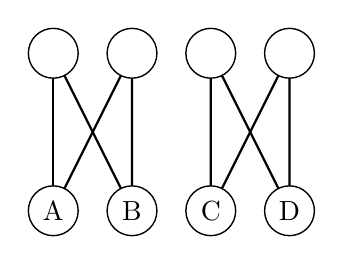
\begin{tikzpicture}[scale=0.10]
%\SetVertexNormal
\SetUpEdge[labelstyle={draw}]
\Vertex[x=0,y=0]{A}
\Vertex[x=10,y=0]{B}
\Vertex[x=20,y=0]{C}
\Vertex[x=30,y=0]{D}
\SetVertexNoLabel
\Vertex[x=0,y=20]{E}
\Vertex[x=10,y=20]{F}
\Vertex[x=20,y=20]{G}
\Vertex[x=30,y=20]{H}
\Edges(A, F, B, E, A)
\Edges(C, H, D, G, C)
\end{tikzpicture}
&
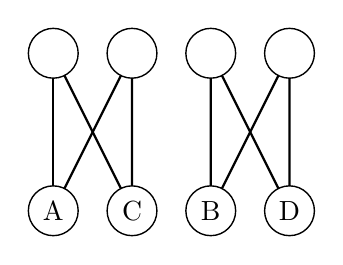
\begin{tikzpicture}[scale=0.10]
%\SetVertexNormal
\SetUpEdge[labelstyle={draw}]
\Vertex[x=0,y=0]{A}
\Vertex[x=10,y=0]{C}
\Vertex[x=20,y=0]{B}
\Vertex[x=30,y=0]{D}
\SetVertexNoLabel
\Vertex[x=0,y=20]{E}
\Vertex[x=10,y=20]{G}
\Vertex[x=20,y=20]{F}
\Vertex[x=30,y=20]{H}
\Edges(A, G, C, E, A)
\Edges(B, H, D, F, B)
\end{tikzpicture}
\end{tabular}
%\includegraphics[scale=0.5]{4cubefold}
\caption{Taking the product of the two adinkras here with the following identification gives a non-disconnected adinkra with 16 vertices. \label{fig:disconnected}}
\end{center}
\end{figure}



\section{ESDE Codes}

Define a \emph{even-split doubly-even (ESDE) code} to be a doubly-even code isomorphic to a direct sum $C_L \oplus C_R$ of even codes. Recall that $1$-d chromotopologies are in bijection with quotients of the hamming cube $I^n$ by a doubly-even code $L$, so any adinkra $A$ has a well-defined associated code $L(A)$ that is uniquely determined by just the graph structure of the adinkra. Our goal is to show that ESDE codes are exactly the codes that appear for $2$-d adinkras. To do this, we introduce a special family of $2$-d adinkras.

For an $1$-d adinkra $A$ with grading function $g$, let $\val(A)$, the \emph{valise} of $A$, be defined as a $1$-d adinkra $A'$ identical to $A$ except for its grading function $g'$, defined as $g'(v) = 0$ if $g(v) \in 2\ZZ$ and $1$ otherwise. It is easy to see that $\val(A)$ is also an adinkra. Similarly, for any $2$-d adinkra $A$ with bigrading function $g$, there is a unique $2$-d adinkra $A'$ with the same chromotopology as $A$ such that $(A')_L^0 = \val(A_L^0)$ and $(A')_R^0 = \val(A_R^0)$, defined with a bigrading function $g'(v) = (x', y')$, where $x', y' \in \{0,1\}$ depending on $x$ and $y \pmod(2)$ respectively given $g(v) = (x,y)$. We similarly denote $A'$ by $\val(A)$ and call such an adinkra a \emph{valise} ($2$-d) adinkra. Equivalently, a valise adinkra is one where the supporting rectangle is a $2 \times 2$ square, and any $2$-d adinkra could be put into a valise form. 

\begin{figure}[htb]
\begin{center}

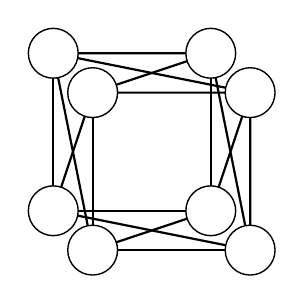
\begin{tikzpicture}[scale=0.10]
%\SetVertexNormal
\SetVertexNoLabel
\SetUpEdge[labelstyle={draw}]
\Vertex[x=0,y=0]{A}
\Vertex[x=-5,y=5]{H}
\Vertex[x=0,y=20]{C}
\Vertex[x=-5,y=25]{B}
\Vertex[x=15,y=5]{D}
\Vertex[x=20,y=0]{E}
\Vertex[x=20,y=20]{G}
\Vertex[x=15,y=25]{F}
\Edges(A,B,G)
\Edges(B,H,C)
\Edges(G,D)
\Edges(C,A,D,H,E,A)
\Edges(D,F,C,G,E,F,B)
\end{tikzpicture}
\caption{A valise $2$-d adinkra that cannot be put into non-valise form.\label{fig:tight valise}}
\end{center}
\end{figure}

\begin{thm}
\label{thm:esde}
For a code $L \subset \ZZ_2^n$, there exists a $2$-d adinkra $A$ with $L(A) = L$ if and only if $L$ is a ESDE code.
\end{thm}
\begin{proof}
Suppose $L(A) = L$ for some $2$-d adinkra $A$. We know that $L$ is doubly-even. Consider any codeword $l \in L$. Starting at $\overline{0} \in A$, moving by a path corresponding to $l$ must end up back at $\overline{0}$. In particular, it must use an even number of left-moving (resp. right-moving) edges since each of which changes the $x$-coordinate (resp. $y$-coordinate) by $1$ in absolute value. Thus, $L$ must be ESDE.

Now, take an ESDE code $L$. $L$ is doubly-even, so there exists a $1$-d adinkra $A$ with code $L(A) = L$. We can assume $A$ is a $1$-d valise by taking $A = \val(A)$ if necessary, which does not change the code. Now, any vertex $v \in A$ corresponds to an equivalence class $c+L \subset \ZZ_2^n.$ consider the function $g'\colon V(A) \rightarrow \{0,1\}$ that sends $v$ to $(x,y)$, where $x$ (resp. $y$) corresponds to the parity of the weight of the left-moving colors of any element in $c+L$. The fact that $L$ is ESDE precisely makes this notion well-defined. Since $g'$ gives $A$ a bigrading, $A$ is realizable as a $2$-d valise adinkra $A$ with code $L$, so we are done. 
\end{proof}


\appendix
\section{Equivalence with other notions of $2$-d Adinkras}


If I read Tristan's stuff right, we can completely translate the combinatorial rules to: a \emph{2-d adinkra} (of dimension $n$) is a finite simple connected graph $A$ such that:
\begin{itemize}
\item It is an $1$-d adinkra (with the associated ranking, dashing, etc.).
\item It has $p + q = n$ colors, where the first $p$-colors are called ``left-moving'' and the second $q$-colors are called ``right-moving.''
\item A coherence condition: for any cycle, we imagine the following sum: going up (here ``up'' comes from the grading we have from the engineering dimension in our ranking for the $1$-d adinkra) a left-handed edge adds $-1$, and going up a right-handed edge adds $1$; going down the edges give contributions with opposite signs. The sum of this around any cycle must be $0$. (in particular, this rules out things like ambidextrous bow-ties)
\end{itemize} 

Assuming I interpreted these rules correctly, now I can do combinatorics without needing any physics.

%%

The first structural fact we can impose is a bi-grading that is compatible with the grading we already have from the $1$-d adinkra structure, in the sense that the $1$-d grading is simply one of the coordinates of our bi-grading.

\begin{prop}
A $1$-d adinkra can be extended to a $2$-d adinkra if and only if the $1$-d adinkra has a \emph{bigrading} to $\ZZ^2$. This is a map $g: V \rightarrow \ZZ^2$, such that all left-moving edges correspond to displacements of $(0, 1)$ and right-moving edges correspond to displacements of $(1, 0)$.
\end{prop}

\begin{proof}
Proof delayed until talking more with Kevin and Tristan about the easiest way to write things up to avoid reinventing wheels.
\end{proof}

\section{Misc. (unorganized)}

\begin{cor}
\label{cor:factorization-connected-components}
Consider the vertex $\overline{0} \in A$. Let the connected component of $A_L$ (resp. $A_R$) that $\overline{0}$ belongs to be labeled $A_L^0$ (resp. $A_R^0$). The adinkra $A$ is uniquely determined\footnote{This is fairly nuanced; we need to know not just the shape of $A_L^0$ and $A_R^0$, but also their vertices} by $A_L^0$ and $A_R^0$.
\end{cor}
\begin{proof}
Consider the color sequence $d$ of any path from $\overline{0}$ to a vertex $v$. We can permute the sequence so that the left-moving colors all occur before the right-moving colors. Thus, we first make some moves in $A_L^0$, then by Proposition~\ref{prop:kevin} we make the remaining moves in a copy of $A_R^0$. 
\end{proof}


\begin{cor}
\label{cor:valise factorization}
A valise $2$-d adinkra $A$ of type $(n,k)$ is uniquely determined by $B_L(A)$, $B_R(A)$, and an identification of $V(B_L(A), 0)$ and $V(B_R(A), 0)$. Furthermore, $|B_L(A)| = |B_R(A)| = 2^{n-k-1}$.
\end{cor}


\begin{prob}
What are all the $2$-d adinkras $A$ with the same valise adinkra $\val(A)$? Not all lifts are possible. For example, the adinkra in Figure~\ref{fig:tight valise} cannot be lifted to any non-valise form!
\end{prob}


\bibliographystyle{abbrv}
\bibliography{Adinkras}

Here are some other problems:
\begin{prob}
Given two valise $1$-d adinkras $B_L(A)$ and $B_R(A)$ of equal size, what identifications of $V(B_L(A), 0)$ and $V(B_R(A), 0)$ are possible?
\end{prob}
\begin{proof}
Data: if we have $\{0,1\} \cup \{2,3\}$ on one side, the other side must be $\{0,2\} \cup \{1, 3\}$.
\end{proof}

\com{There are two kinds of quotienting that we can think of: one quotient is directly quotienting the mega hypercube adinkra by a ESDE code; one quotient is given the valise adinkra with associated $B_L(A)$, $B_R(A)$ each with $2^{d+1}$ vertices, the necessary $d$-dimensional quotienting that occurs when we naively tensor the two parts (which gives $2^{2d}$ vertices in each corner, for $2^{2d+2}$ total vertices, when in the end we just want $2^{d+2}$ vertices.}



\end{document}